% Systemdokumentation OOP3
% Unterlage für Studenten als Leitfaden für die Erstellung einer SystemDoku
% 17. Oktober 2022
% ---------------------------------------------------------------------------



% Dokumentklasse
% --------------
\documentclass[12pt,naustrian,a4widepaper]{scrartcl}   
% article style
%   - 11pt Schriftgroesse
%   - new austrian (neue Rechtschreibung)
%   - Papierformat A4
%   - pdf-hyperlinks


% Packages
% --------
\usepackage[utf8]{inputenc}  % fuer Umlaute, Ü
\usepackage[T1]{fontenc}
\usepackage{a4wide}
\usepackage{times}      % Times Schriften (zusammen mit fontencoding, s.o.)
\usepackage{pdflscape}
\usepackage{babel}
\usepackage{graphicx}	  % für das Einbinden von Grafiken
\usepackage{color}      % für färbigen Text
\usepackage{framed}     % für (Text-) Rahmen
\usepackage{fancyhdr}   % für Kopf- und Fusszeilen
\usepackage{listings}   % für den Sourcecode
\usepackage{pdfpages}
\usepackage{geometry}

\pagestyle{fancy}       % Kopf- / Fusszeile aktivieren

\definecolor{failred}{rgb}{0.7, 0.0, 0.0}
\definecolor{okgreen}{rgb}{0.0, 0.5, 0.0}
\definecolor{gray}{rgb}{0.0, 0.5, 0.0}

\lstdefinelanguage{TestOutput}{
    morekeywords={},
    morecomment=[l]{//},
    morestring=[b]",
    sensitive=false,
}

\lstdefinestyle{teststyle}{
    language=TestOutput,
    basicstyle=\ttfamily\footnotesize,
    keywordstyle=\color{black},
    commentstyle=\color{gray},
    stringstyle=\color{black},
    showstringspaces=false,
    breaklines=true,
    frame=single,
    numbers=left,
    numberstyle=\tiny\color{gray},
    postbreak=\mbox{\textcolor{red}{$\hookrightarrow$}\space},
    literate={OK}{{\textcolor{okgreen}{OK}}}2
             {Fail}{{\textcolor{failred}{Fail}}}4,
}

\lstdefinestyle{cppstyle}{
  language=C++,
  basicstyle=\ttfamily\tiny,
  keywordstyle=\color{blue},
  commentstyle=\textcolor{okgreen},
  stringstyle=\color{red},
  numbers=left,
  numberstyle=\tiny\color{gray},
  stepnumber=1,
  breaklines=true,
  frame=single
}


% Seitenspiegel
% -------------

\typearea{8}	% Festlegung des Seitenspiegels gem. Koma. 4..groß, 9..klein


% Kopfzeile
% ---------
\lhead{{\footnotesize{s. Offenberger, S. Vogelhuber}}}   %  (links)
\chead{{\footnotesize{Systemdokumentation - Fuhrpark}}} %  (mitte)
\rhead{{\footnotesize{Seite \thepage}}}      %  (rechts)

% Fusszeile
% ---------
\lfoot{}  % links
\cfoot{}  % mitte 
\rfoot{}  % rechts

% Absatzformatierung
% ------------------
\setlength{\parindent}{0cm}   % Einrückung der 1. Zeile jedes Absatzes
\setlength{\parskip}{10pt}    % Abstand zwischen den Absätzen


% Package für Hyperlinks (mit pdf-Optionen)
% -----------------------------------------
\usepackage[
urlcolor=blue,		% blaue weblinks
linkcolor=black,	% interne Links sind schwarz
colorlinks=true,        % links werden eingefärbt
pdfstartview=FitH,      % PDF-Anzeige: Fensterbreite
pdfborder={0 0 0},      % keine Umrandung um links
pdftitle   ={Systemdokumentation},% Referenzen in der Pdf-Datei
pdfauthor  ={M. Mustermann, S. Sorglos},
pdfsubject ={Systemdoku},
pdfcreator ={Der Creator},
pdfproducer={Der Producer},
pdfkeywords={Dokumentation, Systemdokumentation}
]{hyperref}


% Beginn des Dokumentes
% ---------------------
\begin{document}

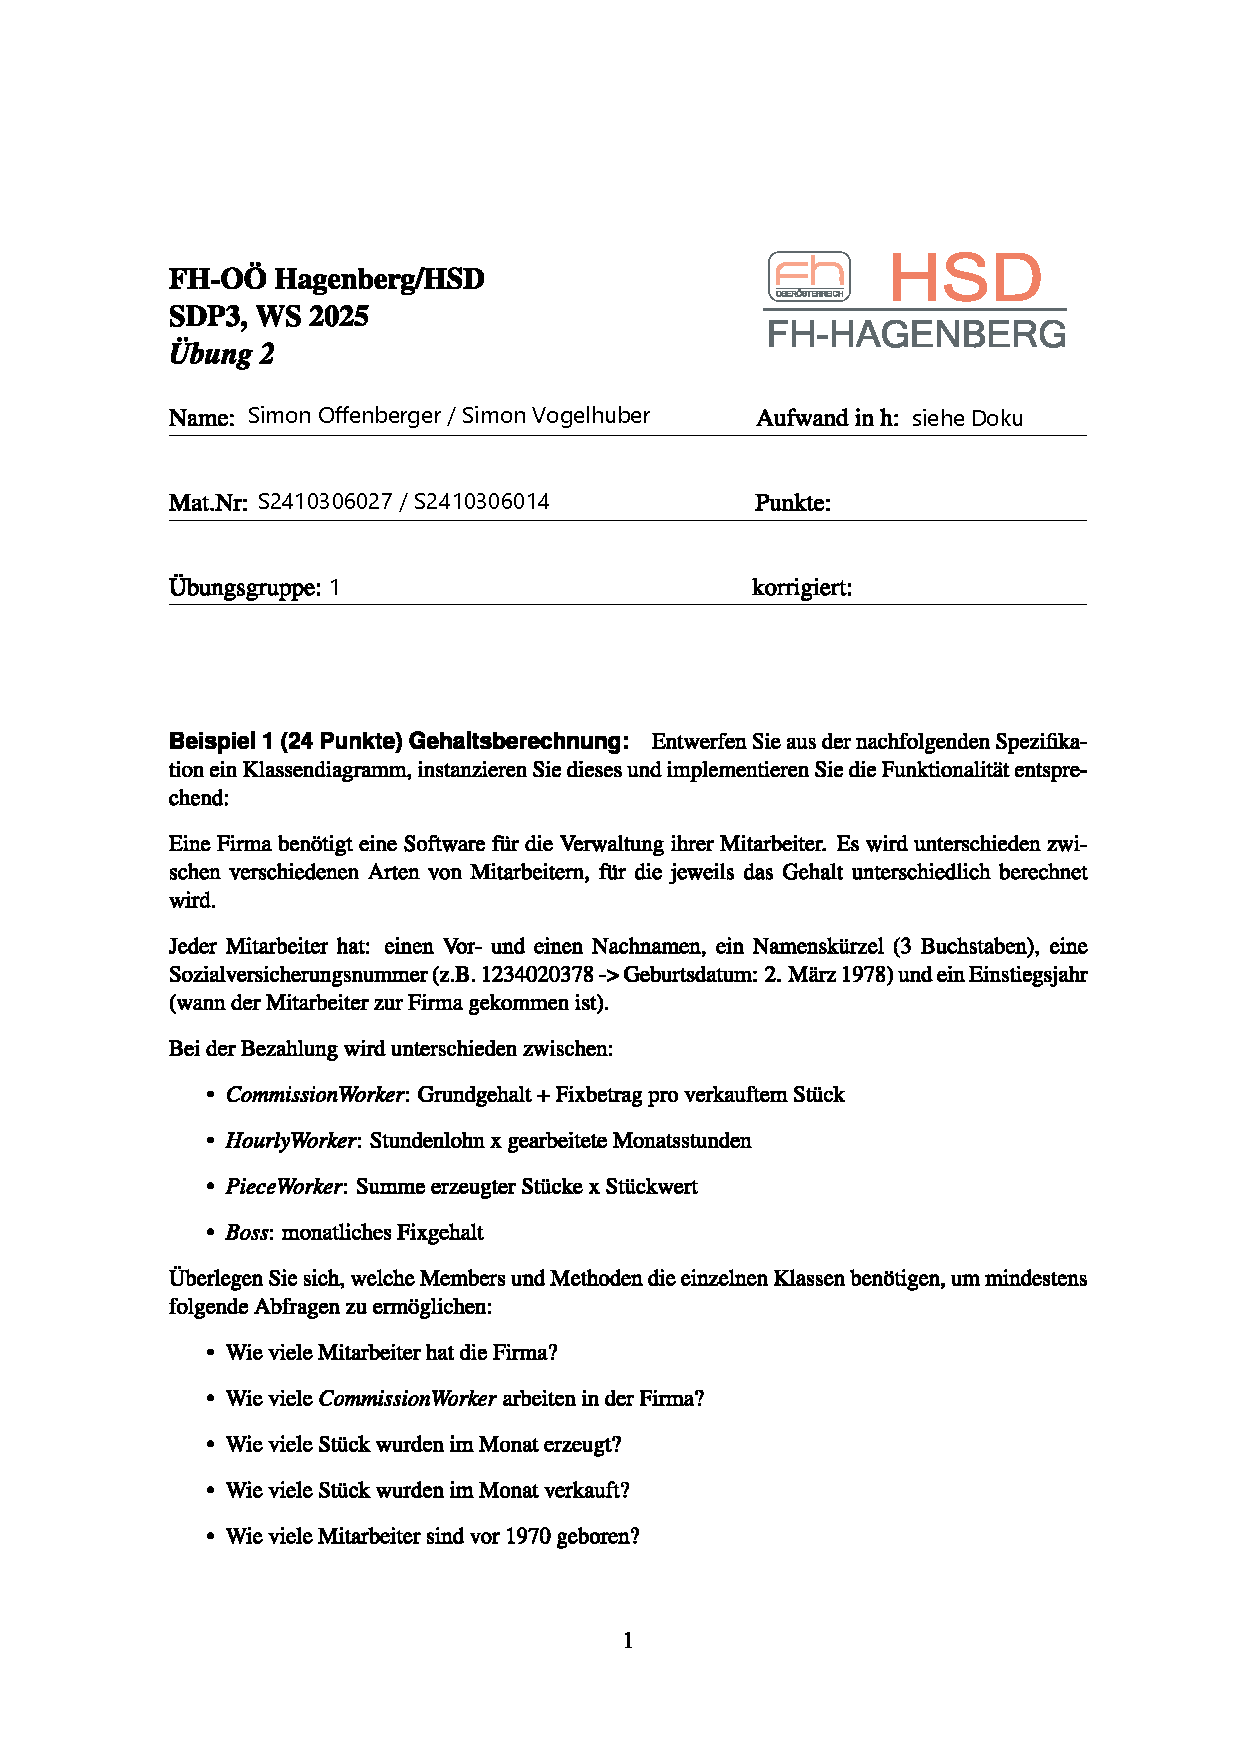
\includepdf[pages = 1-2]{Uebung02_Deckblatt.pdf}

\selectlanguage{naustrian}   % oder "american" für engl. Texte

% Titelblatt
% ----------
\title {\vspace{1cm}
       
\includegraphics[width=8cm]{./Images/FhOOeLogoOkt2009_HSD_Rot_pastell}\\
       \vspace{2cm}
       {\textbf{Systemdokumentation\\Projekt Gehaltsberechnung}}\\
       \vspace{5mm}
       {\small{Version 1.0}}\\
       \vspace{5mm}
}

\author{\small{S. Offenberger, S. Vogelhuber}}
\date  {\small{Hagenberg, \today}}
\maketitle

%\begin{abstract}
%Dieses Dokument zeigt den prinzipiellen Aufbau einer Systemdokumentation für Software-Projekte. Die einzelnen Kapitel sind mit Kommentaren versehen, welche die Struktur und den Inhalt erläutern. 
%\end{abstract}

\clearpage

% Inhalts-, Tabellen- und Bildverzeichnis (werden generiert)
% ----------------------------------------------------------
\tableofcontents
% \listoftables
% \listoffigures
\clearpage



\section{Organisatorisches}

\subsection{Team}
\begin{itemize}
	\item Simon Offenberger, Matr.-Nr.: S2410306027, E-Mail: Simon.Offenberger@fh-hagenberg.at
	\item Simon Vogelhuber, Matr.-Nr.: S2410306014, E-Mail: s2410306014@fhooe.at	
\end{itemize}

\subsection{Aufteilung der Verantwortlichkeitsbereiche}
\begin{itemize}
	\item Simon Offenberger
		\begin{itemize}
			\item Design Klassendiagramm
			\item Implementierung und Test der Klassen: 
			\begin{itemize}
				\item Company
				\item Company Interface
				\item Client
			\end{itemize}
			\item Implementierung des Testtreibers
			\item Dokumentation
		\end{itemize}
	\item Simon Vogelhuber
		\begin{itemize}
			\item Design Klassendiagramm
			\item Implementierung und Komponententest der Klassen: 
			\begin{itemize}
				\item Employee
				\item Boss
				\item ComissionWorker
				\item PieceWorker
				\item HourlyWorker
			\end{itemize}
			\item Implementierung des Testtreibers
			\item Dokumentation
		\end{itemize}	
\end{itemize}

\subsection{Aufwand}
	
	\begin{itemize}
		\item Simon Offenberger: geschätzt 10 Ph / tatsächlich 7 Ph
		\item Simon Vogelhuber:  geschätzt 10 Ph / tatsächlich 8,5 Ph
	\end{itemize}

\clearpage
\section{Anforderungsdefinition (Systemspezifikation)}
In diesem Projekt geht es darum die Mitarbeiter eines Unternehmens zu verwalten und deren Gehälter zu berechnen.
Es gibt verschiedene Arten von Mitarbeitern, welche unterschiedliche Gehaltsberechnungen haben. 
Der Zugriff auf die Mitarbeiter soll über eine gemeinsame Schnittstelle erfolgen.
\\
\\
\textbf{Funktionen der Firmenschnittstelle}
\begin{itemize}
	\item Zugriff auf die wichtigsten Mitarbeiter und Firmendaten
\end{itemize}

\textbf{Funktionen der Firma}
\begin{itemize}
 \item Abfage nach der Anzahl der Mitarbeiter.
 \item Abfage nach der Anzahl eines Mitarbeitertyps in der Firma
 \item Wie viele Stück wurden im Monat erzeugt?
 \item Wie viele Stück wurden im Monat verkauft?
 \item Wie viele Mitarbeiter sind vor einem bestimmten Datum geboren?
 \item Wie hoch ist das Monatsgehalt eines Mitarbeiters?
 \item Gibt es einen Mitarbeiter zu einem gegebenen Namenskürzel?
 \item Welche(r) Mitarbeiter ist/sind am längsten in der Firma?
 \item Ausgabe aller Datenblätter der Mitarbeiter
\end{itemize}

\textbf{Funktionen der Mitarbeiter}
\begin{itemize}
	\item Speichern von Mitarbeiterdaten.
	\begin{itemize}
		\item Name
		\item Namenskürzel
		\item Sozialversicherungsnummer
		\item Einstiegsjahr
		\item Geburtsjahr
	\end{itemize}
	\item Berechnung des Gehalts je nach Mitarbeiterklasse.
	\item Ausgabe von Mitarbeiterinformationen in form eines Datenblatts.
\end{itemize}

\clearpage
\section{Systementwurf}

\subsection{Klassendiagramm}
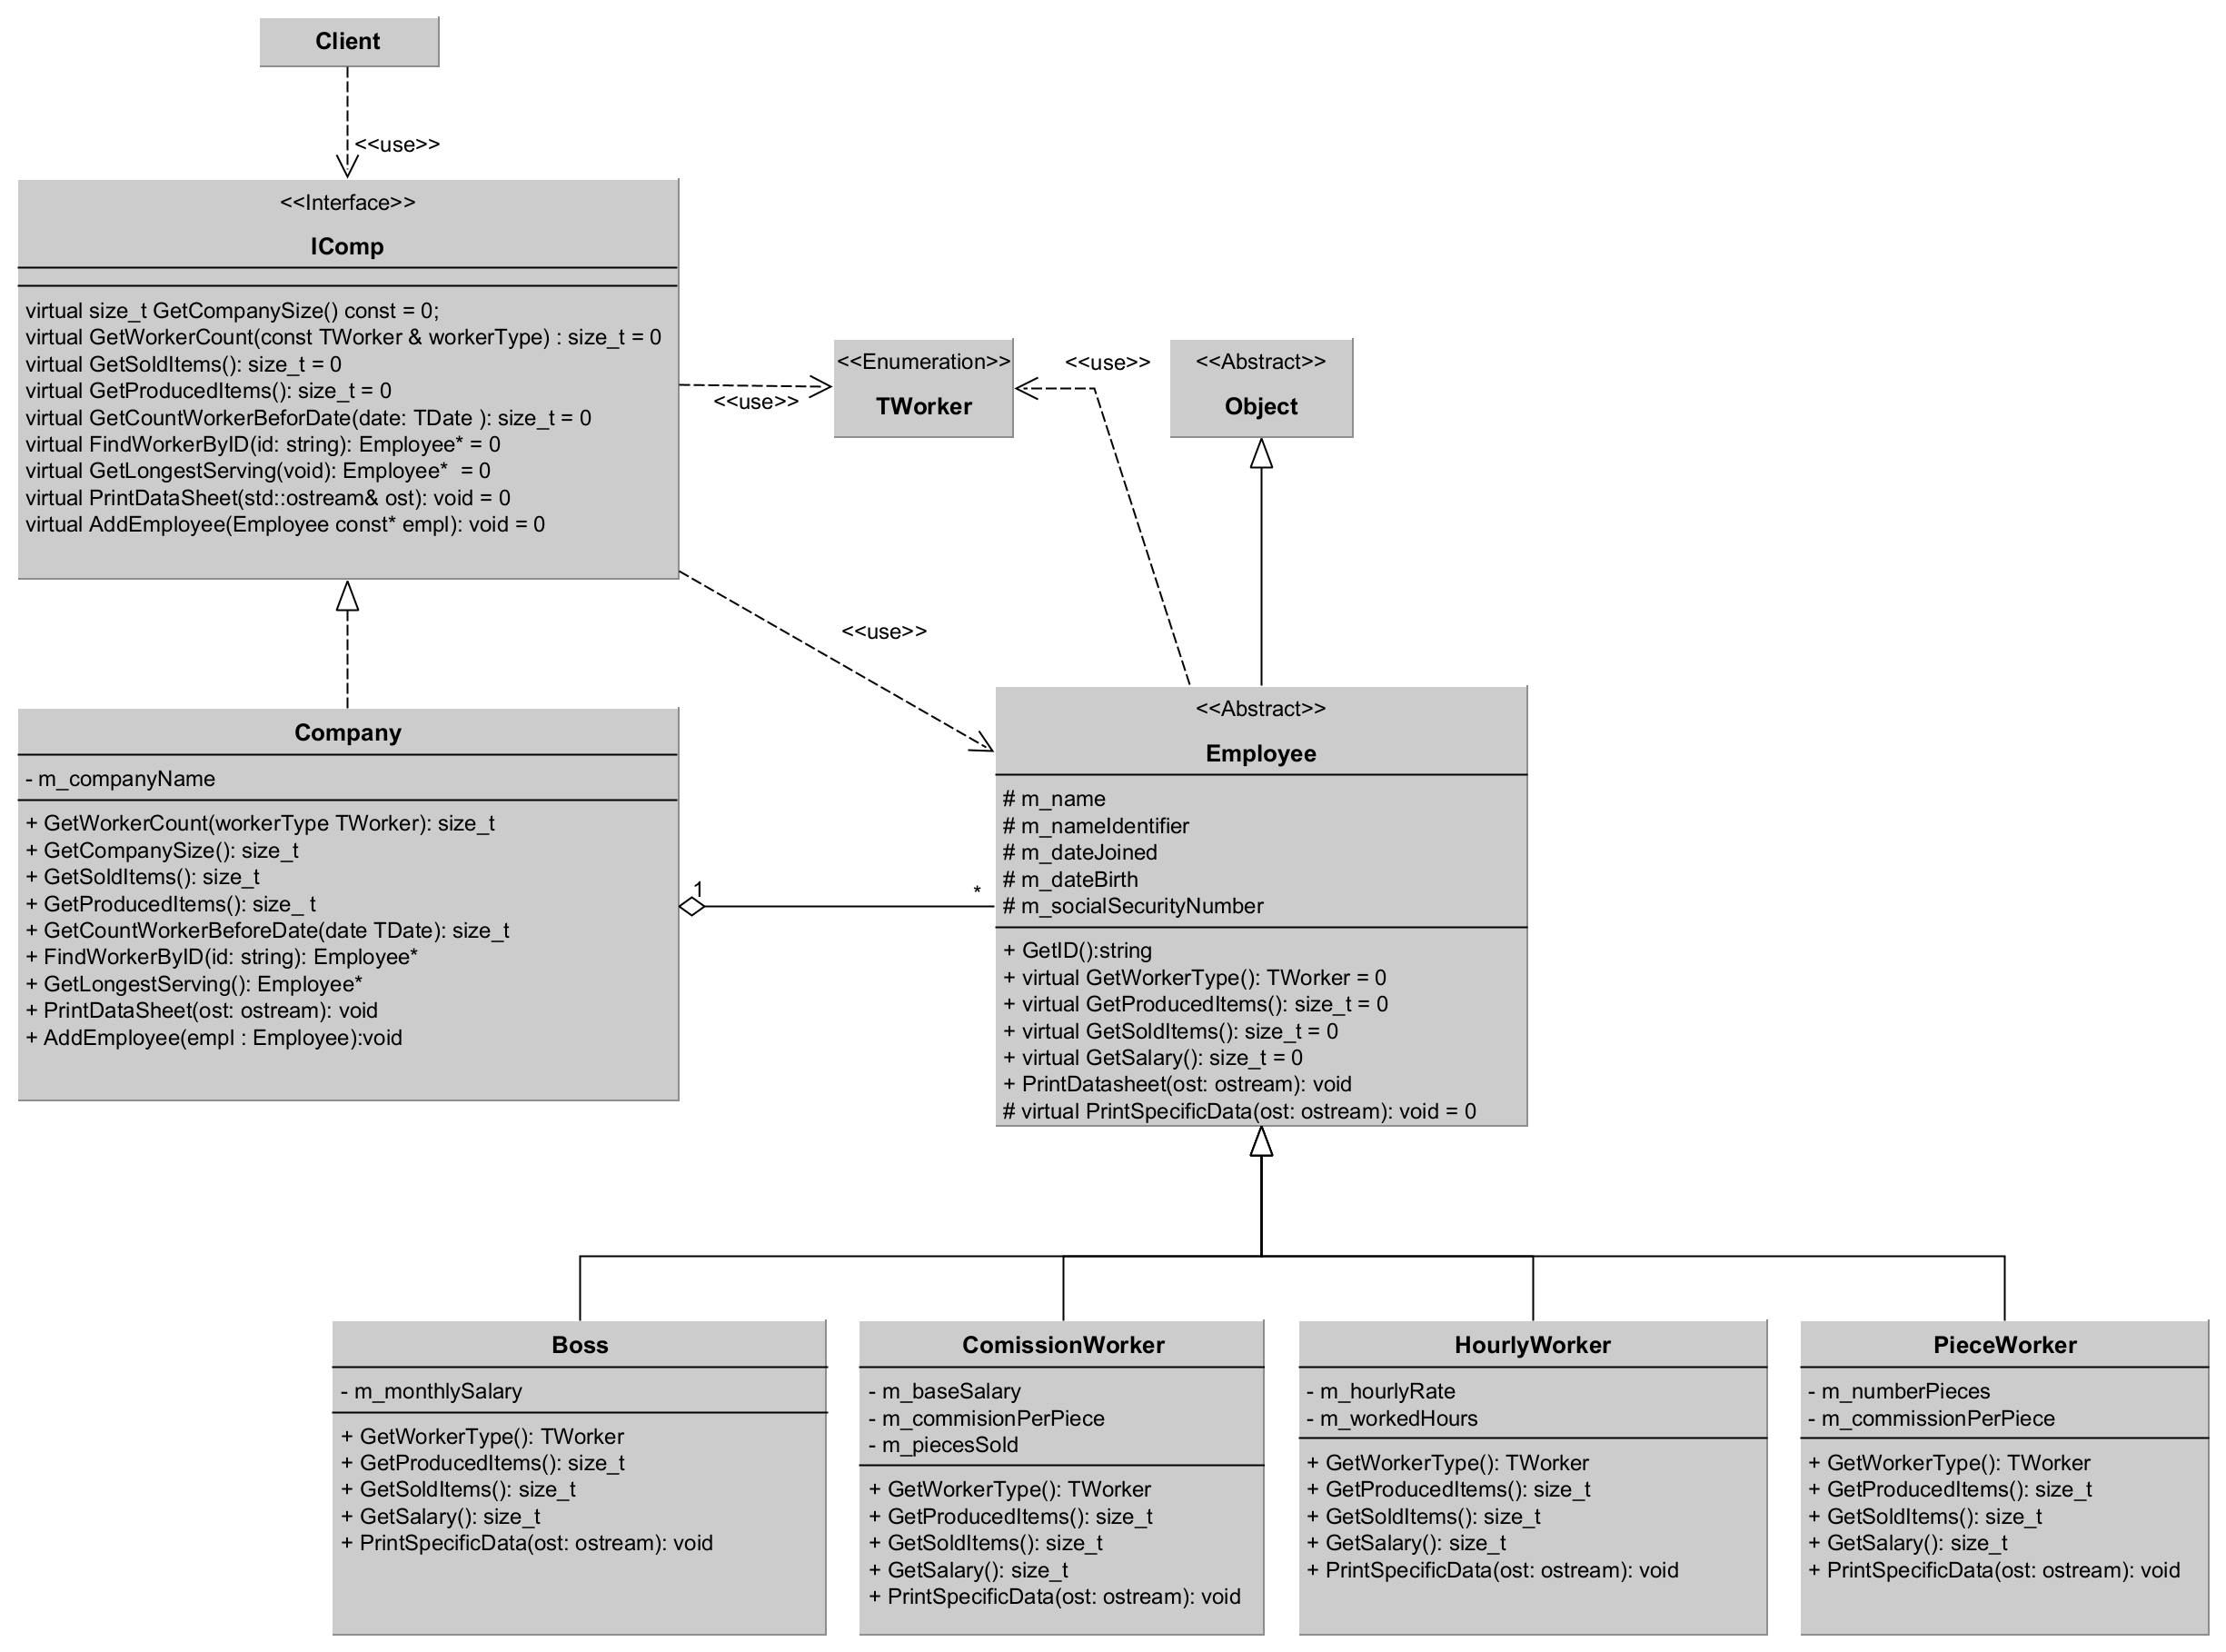
\includegraphics[width=14cm]{./Images/UML_Diagramm.png}
\newpage

\subsection{Designentscheidungen}

Das Interface \textbf{ICompany} wurde erstellt, um dem zugreifenden \textbf{Client} eine Schnittstelle zur Verfügung zu stellen.
Dadurch kann sich der Client auf die Schnittstelle konzentrieren und muss sich nicht um die Implementierungsdetails der Firma kümmern.
\\
\\
Die Firma speichert einen polymorphen Container, der Objekte der abstrakten Klasse \textbf{Employee} verwaltet.
Bei dem Container wurde eine Map verwendet, da die Mitarbeiter über eine eindeutige ID angesprochen werden können.
Somit ist auch das Suchen nach einem Mitarbeiter sehr performant gelöst.
\\
\\
Die Klasse \textbf{Employee} ist abstrakt, da es keine generellen Mitarbeiter geben soll, sondern nur spezielle Arten von Mitarbeitern.
Die einzelnen Mitarbeiter speichern Daten, die für die Gehaltsberechnung notwendig sind. 
Die Gehaltsberechnung wird über eine virtuelle Funktion realisiert, die in den abgeleiteten Klassen überschrieben wird.
Weiters soll die Ausgabe eines Datenblatts zu jedem Mitarbeiter möglich sein dies wurde mittels \textbf{Template Methode Pattern} gelöst!
\\
\\
Das Enum mit dem Mitarbeitertypen \textbf{TWorker} wurde eingebaut, da die Company den Typen des Mitarbeiters kennen muss, um den Mitarbeiter korrekt zu verwalten.
Hierbei wurde aktiv auf RTTI verzichtet, um die Kopplung zwischen Company und den konkreten Klassen die von Employee ableiten zu reduzieren.
Weiters wurden die konkreten Mitarbeiterklassen so gestaltet, dass sie ohne großen Aufwand zu testen sind.
Aus diesem Grund werden alle Daten im Konstruktor übergeben und es gibt keine Setter-Methoden.
Würde dieses Design in der Praxis verwendet werden, müsste man noch Setter Methoden hinzufügen.
Da dies hier nicht im Fokus steht, wurde dies nicht umgesetzt.\\
\color{black}

\section{Dokumentation der Komponenten (Klassen)}
Die HTML-Startdatei befindet sich im Verzeichnis \href{run:./../doxy/html/index.html}{./../doxy/html/index.html}


\clearpage
\section{Testprotokollierung}
\lstinputlisting[style=teststyle]{../TestOutput.txt}

\clearpage
\newgeometry{left=1cm,right=1cm,top=2cm,bottom=2cm}
\begin{landscape}

	\section{Quellcode}
	
	\subsection{Object.hpp}
	\lstinputlisting[style = cppstyle]{../Object.hpp}
	\clearpage
	\subsection{Client.hpp}
	\lstinputlisting[style = cppstyle]{../Client.hpp}
	\clearpage
	\subsection{Client.cpp}
	\lstinputlisting[style = cppstyle]{../Client.cpp}
	
	\clearpage
	\subsection{IComp.hpp}
	\lstinputlisting[style = cppstyle]{../IComp.hpp}
	
	\clearpage
	\subsection{Company.hpp}
	\lstinputlisting[style = cppstyle]{../Company.hpp}
	\clearpage
	\subsection{Company.cpp}
	\lstinputlisting[style = cppstyle]{../Company.cpp}
	
	\clearpage
	\subsection{TWorker.hpp}
	\lstinputlisting[style = cppstyle]{../TWorker.hpp}
	
	\clearpage
	\subsection{Employee.hpp}
	\lstinputlisting[style = cppstyle]{../Employee.hpp}
	\clearpage
	\subsection{Employee.cpp}
	\lstinputlisting[style = cppstyle]{../Employee.cpp}
	
	\clearpage
	\subsection{Boss.hpp}
	\lstinputlisting[style = cppstyle]{../Boss.hpp}
	\clearpage
	\subsection{Boss.cpp}
	\lstinputlisting[style = cppstyle]{../Boss.cpp}
	
	\clearpage
	\subsection{HourlyWorker.hpp}
	\lstinputlisting[style = cppstyle]{../HourlyWorker.hpp}
	\clearpage
	\subsection{HourlyWorker.cpp}
	\lstinputlisting[style = cppstyle]{../HourlyWorker.cpp}
	
	\clearpage
	\subsection{PieceWorker.hpp}
	\lstinputlisting[style = cppstyle]{../PieceWorker.hpp}
	\clearpage
	\subsection{PieceWorker.cpp}
	\lstinputlisting[style = cppstyle]{../PieceWorker.cpp}
	
	\clearpage
	\subsection{ComissionWorker.hpp}
	\lstinputlisting[style = cppstyle]{../ComissionWorker.hpp}
	\clearpage
	\subsection{ComissionWorker.cpp}
	\lstinputlisting[style = cppstyle]{../ComissionWorker.cpp}
	
	\clearpage
	\subsection{main.cpp}
	\lstinputlisting[style = cppstyle]{../main.cpp}
	\clearpage
	\subsection{Test.hpp}
	\lstinputlisting[style = cppstyle]{../Test.hpp}
\end{landscape}
\restoregeometry
	% Literaturverzeichnis
	% --------------------
	%\begin{thebibliography}{99}
	%\bibitem{Pomberger} Pomberger G., Blaschek G. : \textit{Software Engineering: Prototyping und objektorientert Software-Entwicklung}. Hanser, 1996
	%
	%\end{thebibliography}
	
	
	% Ende des Dokuments
	% ------------------
\end{document}
